\documentclass[11pt]{article}
\usepackage{amsmath, amssymb}
% \usepackage{natbib}
\usepackage{geometry}
\usepackage{float}
\usepackage[colorlinks=true, linkcolor=blue, citecolor=blue, urlcolor=blue]{hyperref}
\usepackage{setspace}
\usepackage{booktabs}
\usepackage{graphicx}
\usepackage{apacite}
\usepackage{natbib}
\usepackage{siunitx}
\usepackage{empheq}

\bibliographystyle{apacite}

\geometry{margin=1in}

\setstretch{1.2}
 \title{The Impact of Tariffs on Exchange Rates}


\author{
Jason Lu\thanks{International Monetary Fund, Research Department. Email: {\tt jlu2@imf.org}} 
\and 
Dimitre Milkov\thanks{International Monetary Fund, Research Department. Email: {\tt dmilkov@imf.org}}
}

\date{First draft: November 10, 2025 \\ This version: \today}

\begin{document}
\maketitle

\section*{Two-Country, Two-Sector, One-Factor Model}

\paragraph{Basic setup.}
We consider a static two-country, two-sector, one-factor (2c2s1f) model. Countries are indexed by $i \in \{A,B\}$, and goods by $g \in \{T_A, T_B, N\}$, where $T_i$ denotes the tradable good produced in country $i$, and $N$ a non-tradable good consumed only domestically. Labor is the only factor of production and is immobile across countries.

\paragraph{Technology.}
Each good is produced with a linear technology:
\begin{equation}
Y_{T_i} = A_{T_i} L_{T_i}, \qquad 
Y_{N_i} = A_{N_i} L_{N_i}, \qquad
L_{T_i} + L_{N_i} = L_i.
\end{equation}
Here $A_{T_i}$ and $A_{N_i}$ denote sectoral productivities, and $L_i$ is the total labor endowment in country $i$.

\paragraph{Equilibrium wages.}
Under perfect competition and linear production technologies 
$Y_{T_i} = A_{T_i} L_{T_i}$ and $Y_{N_i} = A_{N_i} L_{N_i}$, 
wages in each country satisfy
\begin{equation}
w_i = P_{T_i} A_{T_i} = P_{N_i} A_{N_i}.
\label{eq:wage}
\end{equation}
Hence the equilibrium wage is equalized across sectors within each country and can be expressed as
\[
w_{i,T} = P_{T_i} A_{T_i}, \qquad 
w_{i,N} = P_{N_i} A_{N_i}, \qquad 
w_{i,T} = w_{i,N} = w_i.
\]
Relative prices determine the real exchange rate in each country:
\begin{equation}
q_i \equiv \frac{P_{N_i}}{P_{T_i}} = \frac{A_{T_i}}{A_{N_i}}, 
\qquad i \in \{A, B\}.
\label{eq:real_exchange_rate}
\end{equation}


\paragraph{Household budget constraint.}
Let $C_{T_i i}$ denote country $i$'s consumption of its own tradable good, $C_{T_j i}$ its consumption of the tradable good produced in the other country $j \neq i$, and $C_{N_i}$ its consumption of the local non-tradable. With labor income $w_i L_i$, the household budget constraint in units of country $i$’s currency is
\begin{equation}
w_i L_i 
\;=\; P_{T_i}\, C_{T_i i} 
\;+\; \big(e_i\, P_{T_j}\big)\, C_{T_j i} 
\;+\; P_{N_i}\, C_{N_i},
\qquad i,j \in \{A,B\},\ i \neq j,
\label{eq:budget_i}
\end{equation}
where $e_i$ is the nominal exchange rate defined as units of country $i$’s currency per unit of country $j$’s currency (e.g., $e_A$ units of $A$’s currency per unit of $B$’s currency, so that $e_B = 1/e_A$).

\paragraph{Household demand.}
Let the Cobb--Douglas exponents on the two differentiated tradables be 
$\alpha_{T_A}, \alpha_{T_B} \in (0,1)$ with $\alpha_{T_A} + \alpha_{T_B} < 1$. 
Preferences in each country are given by
\[
U_i = C_{T_A i}^{\alpha_{T_A}}\, C_{T_B i}^{\alpha_{T_B}}\, C_{N_i}^{\,1-\alpha_{T_A}-\alpha_{T_B}},
\]
and we assume that the Cobb--Douglas coefficients are identical across countries.

Given the budget constraint in country $i$’s currency,
\[
w_i L_i \;=\; P_{T_i}\, C_{T_i i} \;+\; \big(e_i\,P_{T_j}\big)\, C_{T_j i} \;+\; P_{N_i}\, C_{N_i},
\qquad i,j\in\{A,B\},\ i\neq j,
\]
Cobb--Douglas demands allocate expenditure shares equal to exponents:
\begin{align}
P_{T_i}\, C_{T_i i} \;=\; \alpha_{T_i}\, w_i L_i, 
\qquad 
\big(e_i P_{T_j}\big)\, C_{T_j i} \;=\; \alpha_{T_j}\, w_i L_i,
\qquad
P_{N_i}\, C_{N_i} \;=\; \big(1-\alpha_{T_A}-\alpha_{T_B}\big)\, w_i L_i.
\end{align}
Hence quantities are
\begin{align}
C_{T_i i} \;=\; \frac{\alpha_{T_i}\, w_i L_i}{P_{T_i}}, 
\qquad
C_{T_j i} \;=\; \frac{\alpha_{T_j}\, w_i L_i}{e_i\, P_{T_j}},
\qquad
C_{N_i} \;=\; \frac{\big(1-\alpha_{T_A}-\alpha_{T_B}\big)\, w_i L_i}{P_{N_i}} .
\end{align}


\paragraph{Non-tradables market clearing.}
For each country $i\in\{A,B\}$,
\begin{equation}
Y_{N_i}=C_{N_i}.
\end{equation}
Using $Y_{N_i}=A_{N_i}L_{N_i}$, $P_{N_i}=w_i/A_{N_i}$, and Cobb--Douglas demand,
\begin{equation}
\frac{L_{N_i}}{L_i}=1-\alpha_{T_A}-\alpha_{T_B},\ \ 
\frac{L_{T_i}}{L_i}=\alpha_{T_A}+\alpha_{T_B}.
\end{equation}

\paragraph{Tradables market clearing.}
For each tradable variety $T_i$ produced only in country $i$,
\begin{equation}
Y_{T_i}=C_{T_i i}+C_{T_i j}, \qquad i,j\in\{A,B\},\ i\neq j.
\end{equation}
Using $Y_{T_i}=A_{T_i}L_{T_i}$ and Cobb--Douglas demands,
\begin{equation}
A_{T_i}L_{T_i}
=\frac{\alpha_{T_i}\, w_i L_i}{P_{T_i}}
+\frac{\alpha_{T_i}\, w_j L_j}{e_j\, P_{T_i}},
\qquad i,j\in\{A,B\},
\label{eq:T_world_clearing}
\end{equation}
where $e_j$ denotes units of country $j$’s currency per unit of country $i$’s currency ($e_i=1/e_j$).

\paragraph{Trade balance.}
Let trade balances be measured in each country’s own currency. For country $i$, exports are $P_{T_i} C_{T_i j}$ and imports are $(e_i P_{T_j}) C_{T_j i}$. The (goods) trade balance condition is
\begin{equation}
\mathrm{TB}_i 
= P_{T_i} C_{T_i j} - \big(e_i P_{T_j}\big) C_{T_j i},
\qquad i,j\in\{A,B\},\ i\neq j.
\end{equation}
Imposing balanced trade, $\mathrm{TB}_i=0$, and substituting Cobb--Douglas demands,
\begin{equation}
P_{T_i} C_{T_i j} = \frac{\alpha_{T_i}\, w_j L_j}{e_j},
\qquad
\big(e_i P_{T_j}\big) C_{T_j i} = \alpha_{T_j}\, w_i L_i,
\end{equation}
so that
\begin{equation}
\mathrm{TB}_i=0 
\ \Longleftrightarrow\ 
\frac{\alpha_{T_i}\, w_j L_j}{e_j}
= \alpha_{T_j}\, w_i L_i,
\qquad i,j\in\{A,B\},\ i\neq j.
\label{eq:TB_condition}
\end{equation}

\paragraph{Equilibrium condition.}
We normalize the prices of both tradable goods to one, $P_{T_A}=P_{T_B}=1$. Under perfect competition wages satisfy $w_A=A_{T_A}$ and $w_B=A_{T_B}$, and Cobb--Douglas preferences imply that the value of expenditure on each tradable variety is proportional to income.  In this environment, market clearing for tradable goods does not impose independent restrictions on the exchange rate: with two countries and two tradable goods, Walras' Law ensures that the two global tradables market-clearing conditions collapse to a single constraint in value.

Once $P_{T_A}$ and $P_{T_B}$ are fixed, the only remaining equilibrium condition is \emph{trade balance}.  For country~$A$, this requires that the value of exports of $T_A$ equals the value of imports of $T_B$. Under the normalization $P_{T_A}=P_{T_B}=1$, trade balance is given by
\begin{equation}
    C_{T_A B} \;=\; e\,  C_{T_B A},
\end{equation}
which determines the equilibrium exchange rate~$e$.

\begin{figure}[h]
    \centering
    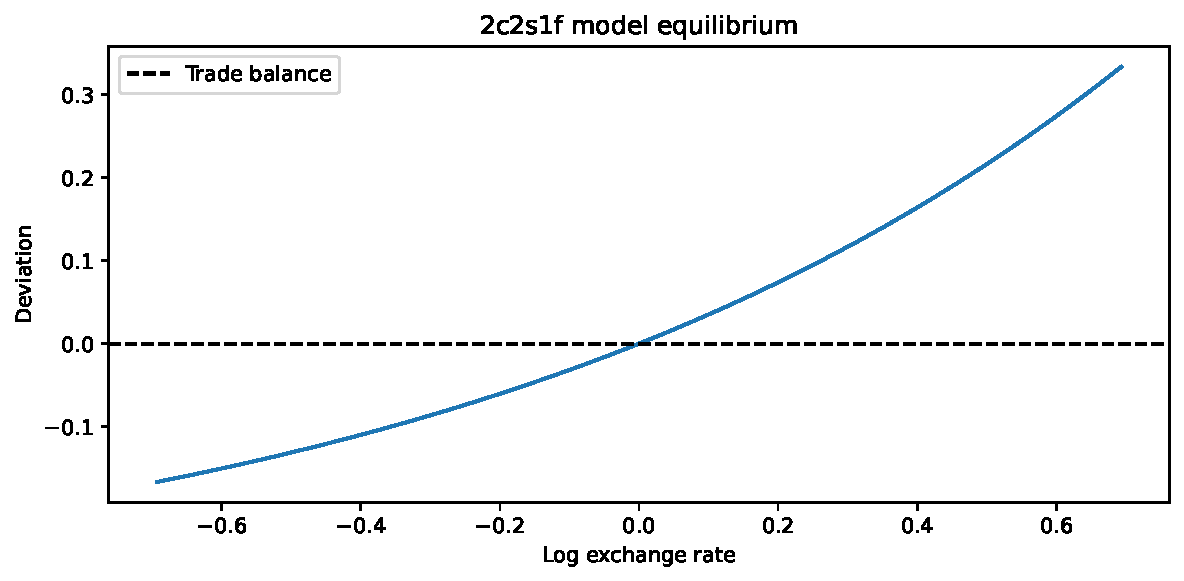
\includegraphics[width=0.8\textwidth]{2c2s1f_eq.pdf}
    \caption{2c2s1f model: trade balance deviation and equilibrium exchange rate.}
    \label{2c2s1f_eq}
\end{figure}

Figure~\ref{2c2s1f_eq} shows the deviation from trade balance as a function of the exchange rate, where equilibrium occurs when the trade balance deviation crosses the zero line, and $A_{N_i} = A_{T_i} = 1$, $\alpha_{T_i} = \alpha_{N} = 1/3$, with normalization $P_{T_A}=P_{T_B}=1$. In this example, the equilibrium exchange rate is $e=1$.

\subsection*{Adding Tariffs}

We now introduce an ad valorem tariff $\tau \ge 0$ levied by country~A on imports of the tradable good~$T_B$.  Let $P_{T_A}=P_{T_B}=1$ remain the numeraire normalization.  The tariff raises the consumer price of $T_B$ in~A to $(1+\tau)e$, where $e$ is the nominal exchange rate (units of A’s currency per unit of B’s currency).  Producers in country~B continue to receive the world price of~$1$, so the price wedge $(1+\tau)e - e = \tau e$ is collected as tariff revenue.

Country~A's household budget constraint becomes
\begin{equation}
    w_A L_A + T_A^\text{rev}
    = C_{T_A A} + (1+\tau)e\, C_{T_B A} + P_{N_A} C_{N_A},
\end{equation}
where $T_A^\text{rev}=\tau e\, C_{T_B A}$ denotes tariff revenue, which we assume is rebated lump-sum to households in~A. Cobb--Douglas preferences still imply expenditure shares proportional to $(\alpha_{T_A},\alpha_{T_B},1-\alpha_{T_A}-\alpha_{T_B})$, but the higher consumer price of~$T_B$ reduces the quantity of~$T_B$ imported by~A.

Solving for demand as a function of parameters, prices, exchange rates, and tariff rates, gives:
\paragraph{Demand in country~A:}
\begin{align}
C_{T_A A} &= \alpha_{T_A}\, I_A, \\[6pt]
C_{T_B A} &= \alpha_{T_B}\, \frac{I_A}{(1+\tau)\, e_{AB}}, \\[6pt]
C_{N_A}   &= \alpha_N\, \frac{I_A}{P_{N_A}}.
\end{align}

\paragraph{Demand in country~B:}
\begin{align}
C_{T_A B} &= \alpha_{T_A}\, \frac{w_B L_B}{e_{BA}}, \\[6pt]
C_{T_B B} &= \alpha_{T_B}\, w_B L_B, \\[6pt]
C_{N_B}   &= \alpha_N\, \frac{w_B L_B}{P_{N_B}}.
\end{align}


\paragraph{Market clearing and equilibrium.}
Tariffs do not affect domestic production decisions in this model. Although the tariff increases household income in country $A$ through rebated tariff revenue, the Cobb–Douglas structure implies that expenditure shares on $T_A$, $T_B$, and $N_A$ remain fixed. On the production side, firms are competitive price takers and use linear technologies, so equilibrium wages satisfy $w_i = P_{T_i} A_{T_i} = P_{N_i} A_{N_i}$. The tariff raises only the consumer price of the imported good $T_B$ in country $A$; it does not change the producer price received by firms in either country. Consequently, domestic wages and relative producer prices are unchanged, leaving the firms' labor demand conditions unaffected. Since sectoral labor allocations depend solely on these producer price ratios and Cobb–Douglas expenditure shares, both $L_{T_i}$ and $L_{N_i}$ remain identical to their free-trade levels, even though the level of household income in $A$ changes.

\begin{figure}[H]
    \centering
    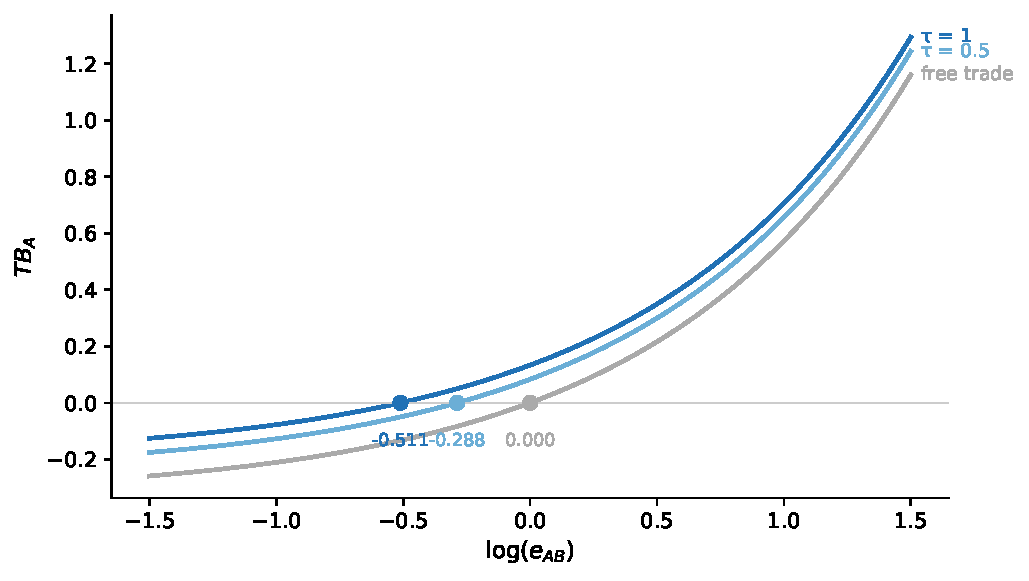
\includegraphics[width=0.8\textwidth]{2c2s1f_with_tariffs_eq.pdf}
    \caption{2c2s1f model with tariffs: trade balance deviation and equilibrium exchange rate.}
    \label{2c2s1f_with_tariffs_eq}
\end{figure}

Despite the addition of tariffs, the trade balance equation is unchanged, and is sufficient to characterize the equilibrium. Figure~\ref{2c2s1f_with_tariffs_eq} shows the deviation from trade balance as a function of the exchange rate subject to different tariff rates. In particular, we see that the equilibrium exchange rate is decreasing in the tariff rate, i.e., when country A raises tariffs, currency A appreciates relative to currency B.

In particular, the analytical expression for the equilibrium exchange rate is given by
\begin{equation}
    e(\tau)
    = \frac{1}{1+\tau(1-\alpha_{T_B})}
      \left( \frac{\alpha_{T_B}}{\alpha_{T_A}} \right)
      \left( \frac{A_{T_A} L_A}{A_{T_B} L_B} \right),
\end{equation}
which is strictly decreasing in the tariff rate~$\tau$ assuming that $\alpha_{T_B}>0$.

\end{document}
